\section{HIERARCHICAL FRAMEWORK AND ROTATION-SYNCHRONIZED WINDOW GUIDANCE}\label{sec:framework}

This section addresses the first question of Section~\ref{sec:mission}. It introduces the hierarchical structure and the interface through which the execution layer serves the decision layer, develops the rotation-synchronized window guidance (RWG) that turns a two-dimensional intent into motion synchronized with the rotating port, and describes the entry logic and the constrained controllers that complete the execution layer. The coupling between the two layers is the subject of Section~\ref{sec:ecc}.

\subsection{Hierarchical Structure and Execution-Layer Interface}\label{sec:integration}

Constrained optimization enforces the constraints of Table~\ref{tab:constraints} explicitly, but in the near field its horizon covers seconds, whereas the value of a decision in Problem~1 depends on whether a pass tens of seconds ahead is used or missed \cite{reiter2026arc,ren2026taes}. A learned policy can represent such long-horizon trade-offs between time, propellant, and opportunity, but learning thrust commands end to end, as in \cite{yang2025taes}, requires extensive interaction and offers limited means to enforce hard constraints \cite{reiter2026arc}. The two roles are therefore assigned to two layers. Once per stage of nominal duration $h$, a learned decision layer issues a stage intent $\ba=[a_{\mathrm{p}},a_{\mathrm{z}}]^{\T}\in\Aset=[-1,1]^{2}$, whose components set the closing pace and the timing of the encounter with the rotating port. An execution layer with fixed parameters converts the intent into constrained motion, decides and plans the entry toward the port, and executes the near-field approach. In the taxonomy of \cite{reiter2026arc}, the decision layer parameterizes an optimization-based executor that is part of the environment during learning. Three design choices shape the structure.

\textit{1) Event-driven macro steps:} A decision is requested at the end of a stage, or earlier when the tracking deviation exceeds $\bar d_{\mathrm{h}}$ and the execution layer switches to hold. Once an entry transfer or the terminal descent has begun, the execution layer continues without further decisions until termination or until the entry is lost. An entry is thus never interrupted by the policy, and the interval between two decisions, called a macro step, has a well-defined outcome: the reward accumulated over it, the successor state, and a termination flag.

\textit{2) Execution modes:} The execution layer operates in the four modes of Table~\ref{tab:modes}, and decisions are taken only in the stage-flight mode $\modeS$ and the hold mode $\modeH$. Translation beyond the range $\rho_{\mathrm{f}}$ is tracked by a feedback law, and the near-field model predictive controller (MPC) acts within $\rho_{\mathrm{f}}$ and throughout the entry transfer $\modeE$ and the terminal descent $\modeD$, where the port-relative constraints become active. A lost entry or an exit from the descent region reverts to $\modeH$.

\textit{3) Multirate operation:} Control and constraint evaluation run every $\Delta t$, mode logic and entry checks every $\Tm$, decisions every stage $h$, and the mode prediction of Section~\ref{sec:screening} covers $\Tp=3h$. The stage is short compared with a pass, so that several decisions precede each pass and the constant-rate prediction \eqref{eq:pred} remains accurate over a stage, and long enough for the attainable velocity change, which grows with $h^{2}$, to reshape the encounter; three stages cover one pass.

\begin{table}
\caption{Execution Modes}
\label{tab:modes}
\tablefont
\begin{tabular*}{\columnwidth}{@{\extracolsep{\fill}}>{\raggedright\arraybackslash}p{4.0pc}>{\raggedright\arraybackslash}p{7.0pc}>{\raggedright\arraybackslash}p{7.0pc}@{}}
\hline
Mode & Entered when & Translation reference\\
\hline
Stage flight $\modeS$ & Stage plan of the new intent is feasible & Stage plan\\
Hold $\modeH$ & Stage plan infeasible, deviation $>\bar d_{\mathrm{h}}$, entry lost, or descent region left & Inertial position at hold onset\\
Entry transfer $\modeE$ & Entry condition \eqref{eq:entry} holds & Entry plan\\
Terminal descent $\modeD$ & $\brhoT\in\Km$, $\rho<\rhos$, or $\brhoT\in\Kset$ with $\rho<\rho_{\mathrm{D}}$ & Lead point on the port axis\\
\hline
\end{tabular*}
\end{table}

The decision layer interacts with the execution layer only through the following interface.

\begin{definition}[Execution-layer interface]\label{def:interface}
Let the decision state $x\in\Xset$ comprise the joint state $X$, the time $t$, the propellant used $\Delta v$, the mission parameters, and the internal state of the execution layer (mode, hold reference, record of the previous stage, and solver warm starts). At a decision state, the execution layer provides:
\begin{enumerate}
\item the macro-step kernel $\PE(x',r\,|\,x,\ba)$ induced by executing an intent $\ba$ from $x$ until the next decision, where $r$ is the reward of the macro step (Section~\ref{sec:mdp});
\item a mode prediction $\Mpred(x,\bb)$ stating whether, when, and at what propellant cost holding an intent $\bb$ would make the execution layer leave stage flight for an entry transfer or the terminal descent within $\Tp$;
\item an execution-feedback vector $\bz(x)$ of opportunity judgments and execution status.
\end{enumerate}
\end{definition}

Because entry transfers and descents run until termination or until the entry is lost, which voids the entry plan, no unfinished entry plan exists at a decision instant, and $x$ determines the evolution of the closed loop over a macro step. Item~1 is what any learning method interacts with; items~2 and~3 are formed from the rules and models of the execution layer itself and are used in Section~\ref{sec:ecc}. The interface does not refer to a particular execution layer; RWG, developed next, is the instance used in this article. Fig.~\ref{fig:framework} shows the resulting architecture.

\begin{figure*}[t]
\centering
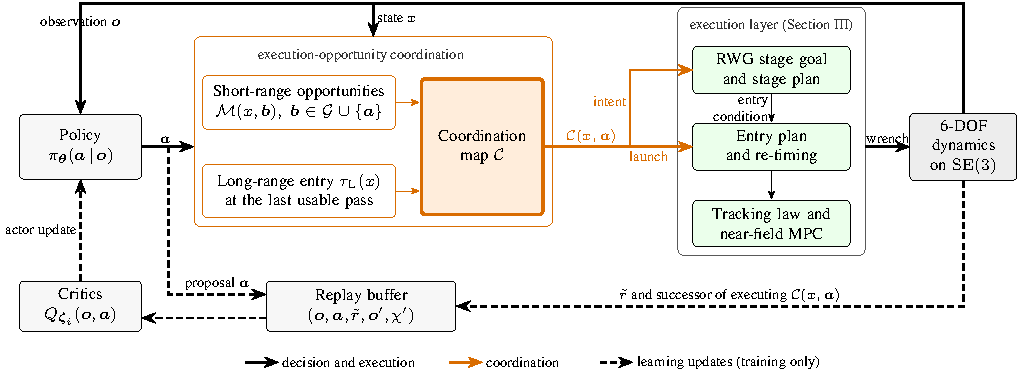
\includegraphics{figures/fig_framework.pdf}
\caption{Execution-aware hierarchical framework. The execution layer exposes the interface of Definition~\ref{def:interface}: the transition of an executed intent, the mode prediction $\Mpred$, and the execution feedback $\bz$. The action-level channel (orange) corrects the proposal $\ba$ into the executed intent $\atil$ in training and execution alike; the state-level channel (blue) feeds $\bz$ to the critics. Dashed paths exist only in training.}
\label{fig:framework}
\end{figure*}

\begin{figure*}[t]
\centering
\begin{minipage}[b]{0.31\textwidth}\centering
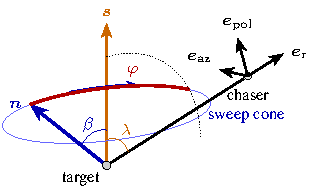
\includegraphics{figures/fig_rwg_a.pdf}\\[2pt]{\footnotesize (a)}
\end{minipage}\hfill
\begin{minipage}[b]{0.35\textwidth}\centering
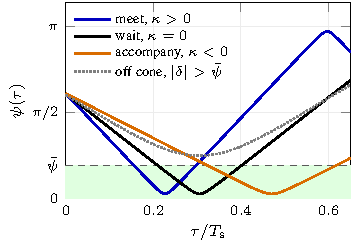
\includegraphics{figures/fig_rwg_b.pdf}\\[2pt]{\footnotesize (b)}
\end{minipage}\hfill
\begin{minipage}[b]{0.33\textwidth}\centering
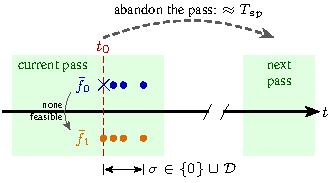
\includegraphics{figures/fig_rwg_c.pdf}\\[2pt]{\footnotesize (c)}
\end{minipage}
\caption{Rotation-synchronized window guidance. (a) Sweep-cone geometry: the port direction $\bn$ rotates about $\bs$ on a cone of half-angle $\beta$; $\lambda$ is the polar angle of the line of sight and $\varphi$ the remaining phase to the pass. (b) Analytic port--line-of-sight angle \eqref{eq:theta} at fixed range under the constant phase rates of Proposition~\ref{prop:rwg}(iii), for $\beta=85^{\circ}$, $\lambda=90^{\circ}$, and $\kappa\in\{0.35,0,-0.35\}$, and for an off-cone line of sight with $|\dlat|>\psig$; the shaded band is the entry gate. (c) Entry re-timing: when the plan arriving at $t_{0}$ is infeasible ($\times$), shifted arrivals with the bounds $\bar f_{0}$ and $\bar f_{1}$ are tried before the pass is abandoned.}
\label{fig:rwg}
\end{figure*}

\subsection{Sweep-Cone Geometry and Rotation-Synchronized Intent}\label{sec:geometry}

RWG addresses Features 1 and 2 of Section~\ref{sec:mission}. Under the prediction \eqref{eq:pred}, the port direction $\bn$ rotates uniformly about $\bs$ and sweeps a cone of half-angle $\beta=\angle(\bn,\bs)$, referred to as the sweep cone. At the relative position $\brho$, a local orthonormal basis is formed by the line-of-sight direction $\er=\brho/\rho$, the unit projection $\epol$ of $\bs$ onto the plane normal to $\er$, and $\eaz=\er\times\epol$, which points toward the oncoming port (Fig.~\ref{fig:rwg}(a)). The geometry is described by the line-of-sight polar angle $\lambda=\angle(\er,\bs)$, the latitude offset $\dlat=\lambda-\beta$, and the phase $\varphi\in[0,2\pi)$ that the port still has to sweep about $\bs$ before it reaches the meridian plane of the line of sight. For the line of sight held fixed, the angle $\psi(\tau)$ between the port direction and $\er$ after a time $\tau$ follows from the spherical law of cosines,
\begin{equation}\label{eq:theta}
\cos\psi(\tau)=\cos\lambda\cos\beta+\sin\lambda\sin\beta\cos(\varphi-\Omega\tau),
\end{equation}
with the phase difference wrapped to $[-\pi,\pi]$. An entry is considered only while $\psi$ is below an entry gate $\psig$.

\begin{lemma}[Passing window]\label{lem:window}
Let $\sin\lambda\sin\beta>0$. If $|\dlat|>\psig$, then $\psi(\tau)>\psig$ for all $\tau$. If $|\dlat|\le\psig$, then $\psi(\tau)\le\psig$ if and only if $|\varphi-\Omega\tau|\le\phw$, where
\begin{equation}\label{eq:halfwidth}
\phw=\arccos\max\Bigl\{-1,\ \frac{\cos\psig-\cos\lambda\cos\beta}{\sin\lambda\sin\beta}\Bigr\};
\end{equation}
each pass thus offers a window of duration $2\phw/\Omega$ centered at $\tau=\varphi/\Omega$, where $\psi$ attains its minimum $|\dlat|$.
\end{lemma}

Lemma~\ref{lem:window} exposes the two levers available to the chaser: the latitude offset decides whether a pass is usable and how closely the port aligns with the line of sight, and the phase decides when the pass occurs. For the spin axes considered, $\dlat=0$ nearly maximizes the window duration (Appendix~\ref{app:proofs}). The time-varying line-of-sight region of multistage MPC approaches to tumbling targets \cite{dong2022aa} plays a similar role, with the difference that here the period of the region is comparable to the deadline, so that a pass is a scarce resource that must be scheduled rather than awaited.

RWG maps the intent to the target velocity at the end of a stage,
\begin{equation}\label{eq:vstar}
\bv^{\star}=-v_{\mathrm{cl}}\,\er+v_{\mathrm{lat}}\,\epol+v_{\mathrm{sw}}\,\eaz,
\end{equation}
with the closing speed $v_{\mathrm{cl}}=v_{0}+v_{\mathrm{a}}a_{\mathrm{p}}$ and the along-sweep speed $v_{\mathrm{sw}}=v_{\mathrm{a}}a_{\mathrm{z}}$ set by the policy, and the latitude speed
\begin{equation}\label{eq:vlat}
v_{\mathrm{lat}}=\sat\bigl(k_{\lambda}\rho\,\dlat;\ \bar v_{\mathrm{lat}}\bigr)
\end{equation}
set by a fixed regulation law with gain $k_{\lambda}$ and saturation level $\bar v_{\mathrm{lat}}$. The three components act on the three quantities of Lemma~\ref{lem:window}.

\begin{proposition}[Nominal window regulation]\label{prop:rwg}
Under the prediction \eqref{eq:pred}, let $\sin\lambda>0$ and resolve the relative velocity as $\bv=v_{\mathrm{r}}\er+v_{\mathrm{pol}}\epol+v_{\mathrm{az}}\eaz$.
\begin{enumerate}
\item The range, the latitude offset, and the phase evolve as
\begin{equation}\label{eq:localkin}
\dot\rho=v_{\mathrm{r}},\qquad \dot{\dlat}=-\frac{v_{\mathrm{pol}}}{\rho},\qquad \dot\varphi=-\Omega-\frac{v_{\mathrm{az}}}{\rho\sin\lambda}.
\end{equation}
\item If $v_{\mathrm{pol}}=v_{\mathrm{lat}}$ follows \eqref{eq:vlat} and $\rho\le\bar\rho_{\mathrm{r}}$, then $|\dlat|$ decreases monotonically, enters the set $|\dlat|\le\bar v_{\mathrm{lat}}/(k_{\lambda}\bar\rho_{\mathrm{r}})$ in finite time, and decays exponentially with rate $k_{\lambda}$ thereafter.
\item If $\rho$ and $\lambda$ are constant and $v_{\mathrm{az}}=v_{\mathrm{sw}}$ is constant with $\kappa=v_{\mathrm{sw}}/(\Omega\rho\sin\lambda)>-1$, then the phase decreases at the rate $\Omega(1+\kappa)$, and the next pass occurs after $\varphi/(\Omega(1+\kappa))$ and lasts $2\phw/(\Omega(1+\kappa))$.
\end{enumerate}
\end{proposition}

The proofs are given in Appendix~\ref{app:proofs}. Proposition~\ref{prop:rwg} assigns one role to each component: $v_{\mathrm{cl}}$ sets the range, $v_{\mathrm{lat}}$ brings the line of sight onto the sweep cone and thereby opens the window of Lemma~\ref{lem:window}, and $v_{\mathrm{sw}}$ places the window in time. Meeting the oncoming port ($\kappa>0$) advances and shortens the pass, accompanying it ($\kappa<0$) delays and lengthens it, and waiting ($\kappa=0$) leaves the natural sweep (Fig.~\ref{fig:rwg}(b)). These are values of one continuous action rather than predefined maneuvers; which of them is preferable depends on the remaining time, the mission, and the propellant, which is the state-dependent decision delegated to learning.

The stage goal is formed from the current state $(\brho,\bv)$ and $\bv^{\star}$ as
\begin{equation}\label{eq:goal}
\begin{aligned}
\bv_{\mathrm{g}}&=\mathcal{P}\bigl(\bv+\sat(\bv^{\star}-\bv;\ \bar v_{\mathrm{st}})\bigr),\\
\brho_{\mathrm{g}}&=\brho+\tfrac{h}{2}(\bv+\bv_{\mathrm{g}}),
\end{aligned}
\end{equation}
where $\bar v_{\mathrm{st}}$ is the velocity change attainable within one stage with a fraction of the planning thrust and $\mathcal{P}$ reduces only the inward radial component of its argument, so that the stage ends at a range of at least $\rho_{\min}>\rhos+\ell_{\mathrm{m}}$ with a radial braking margin of at least $m_{\mathrm{b},\min}$. The operation sphere is thereby entered only through an entry transfer or the terminal descent. The pair $(\brho_{\mathrm{g}},\bv_{\mathrm{g}})$ is the soft terminal target of the stage plan.


\subsection{Dynamic Entry and Entry Re-Timing}\label{sec:entry}

Feature 3 concerns the conversion of a pass into an entry. Both the stage plan and the entry plan are instances of the following subproblem on the double integrator \eqref{eq:di}.

\noindent\textit{Problem~2 (Planning subproblem):} Given the state $(\brho_{0},\bv_{0})$ at time $t$, a horizon $T$ divided into $N$ intervals of length $\Delta t_{\mathrm{pl}}=T/N$, and a thrust bound $\bar f_{\mathrm{pl}}$,
\begin{equation}\label{eq:plan}
\begin{aligned}
\min_{\bff_{0},\dots,\bff_{N-1}}\ \ & L_{\mathrm{f}}(\brho_{N},\bv_{N})+w_{\mathrm{v}}\sum_{n=0}^{N-1}\frac{\norm{\bff_{n}}\Delta t_{\mathrm{pl}}}{\mC}\\
\text{s.t.}\ \ & \eqref{eq:di}\text{ with }\bff\equiv\bff_{n}\text{ on interval }n,\\
& \norm{\bff_{n}}\le\bar f_{\mathrm{pl}},\qquad \rhom\le\rho\le\bar\rho_{\mathrm{pl}},\\
& -\dot\rho\le\vb(\rho-\rhos),\qquad (\brho_{N},\bv_{N})\in\mathcal{X}_{\mathrm{f}},
\end{aligned}
\end{equation}
where the path constraints are imposed at the nodes and at interior points of every interval. The stage plan uses $T=h$, the soft terminal cost $L_{\mathrm{f}}=w_{\rho}\norm{\brho_{N}-\brho_{\mathrm{g}}}^{2}+w_{\mathrm{g}}\norm{\bv_{N}-\bv_{\mathrm{g}}}^{2}$, and no terminal set. The entry plan uses an arrival time $T=\tau$, $L_{\mathrm{f}}=0$, $w_{\mathrm{v}}=1$, and the terminal set that places the chaser at the mouth point $\brhom(t+\tau)=\rhom\hat{\bR}_{\mathrm{T}}(t+\tau)\bnp$ on the port axis outside the operation sphere, moving with it and closing at $v_{\mathrm{in}}$ along the port axis. The keep-out sphere of radius $\rhom$ is nonconvex; following \cite{lian2026asr}, it is linearized at the previous iterate and the problem is solved as a sequence of second-order cone programs. The planning bound $\bar f_{\mathrm{pl}}<\fmax$ leaves a margin for tracking.

While the execution layer is in $\modeS$ or $\modeH$, the entry condition is checked every $\Tm$ once $\rho\le\rho_{\mathrm{E}}$ and the radial braking margin $m_{\mathrm{b}}=\vb(\rho-\rhos)+\dot\rho$ is at least $m_{\mathrm{b},\min}$. The arrival time is the earliest
\begin{equation}\label{eq:entry}
\begin{aligned}
\tau_{\mathrm{e}}=\min\bigl\{\tau\in\Tset:\ &\hat\psi(\tau)\le\psig,\ \ t+\tau\le\te,\\
&\text{Problem~2 is feasible}\bigr\},
\end{aligned}
\end{equation}
where $\Tset$ is a finite set of candidate arrival times, $\hat\psi$ is the angle \eqref{eq:theta} under the prediction \eqref{eq:pred}, and the entry plan uses the bound $\bar f_{0}$. If \eqref{eq:entry} has a solution, the entry transfer starts toward $\brhom(t+\tau_{\mathrm{e}})$. The thresholds $\rho_{\mathrm{E}}$, $\psig$, and $m_{\mathrm{b},\min}$ limit the number of planner calls; safety is defined by Table~\ref{tab:constraints} alone. The latest admissible entry time $\te=\Td-\Tr$ reserves $\Tr$ for the descent.

During the transfer, the entry plan is retained while the tracking deviation stays below $\bar d_{\mathrm{e}}$; otherwise it is re-solved toward the original arrival instant $t_{0}$. If this fails, entry re-timing tries the arrival instants and bounds
\begin{equation}\label{eq:retime}
\begin{aligned}
&(t_{0}+\sigma,\ \bar f_{0}), && \sigma\in\Sigma_{0},\\
&(t_{0}+\sigma,\ \bar f_{1}), && \sigma\in\Sigma_{1}=\{0\}\cup\Sigma_{0},
\end{aligned}
\end{equation}
in this order, subject to $t_{0}+\sigma\le\te$, with shifts $\sigma>0$ in $\Sigma_{0}$ much smaller than $\Ts$ and $\bar f_{0}<\bar f_{1}\le\fmax$. The first feasible candidate is adopted; if none is feasible, the entry is lost and the mode reverts to $\modeH$. Re-timing thus replaces the alternative of abandoning the pass, which costs about one spin period, by a re-plan around the original arrival instant (Fig.~\ref{fig:rwg}(c)).

\begin{remark}\label{rem:retime}
If a feasible entry plan exists with the arrival instant fixed at $t_{0}$, re-timing returns that plan, because its first evaluation is the same convex problem with the same data. For a fixed arrival instant and linearization point, the subproblems with $\bar f_{0}$ and $\bar f_{1}$ differ only in the thrust bound, so the feasible set under $\bar f_{1}$ contains that under $\bar f_{0}$. Re-timing therefore never removes an executable entry. This is a property of the candidate set; it does not imply that the capture rate increases or that a re-timed arrival stays within the same pass.
\end{remark}

\subsection{Constrained Execution Layer}\label{sec:executor}

Beyond $\rho_{\mathrm{f}}$, translation tracks the stage plan in inertial axes by a feedforward and proportional--derivative law, and a pointing controller keeps the boresight on the port. In the terminal descent, the reference is a lead point on the port axis in $\FT$ that advances toward $\bpcap$ at the smaller of the braking-envelope speed and the speed $\fmax/(4\Omega\mC)$ admitted by the Coriolis acceleration.

The near-field MPC computes the full control wrench. Its state is the exponential coordinate of the relative pose and twist $(\bg_{\mathrm{r}},\bxi_{\mathrm{r}})$ in $\FT$, and its prediction model is the relative dynamics linearized at the current state. It minimizes a quadratic cost on the scaled tracking errors and inputs over a horizon of $N_{\mathrm{mpc}}$ control periods, where the translational reference is the plan of the current mode and the attitude reference is the line of sight to the port, switching to the docking attitude in the descent. The constraints comprise the input bounds and the constraints of Table~\ref{tab:constraints} linearized along the predicted trajectory, with the approach cone approximated by a polyhedron and softened by a slack variable. The MPC thus supplies the near-field execution capability, whereas decisions over the horizon of a pass are left to the decision layer.
